\documentclass[11pt]{article}
\usepackage[english]{babel}
\usepackage{minted}
\usepackage{amsmath}
\usepackage{amsthm}
\usepackage{graphicx}
\usepackage{subcaption}
\usepackage{booktabs}
\usepackage[utf8]{inputenc}
% More styles for bullets
\usepackage{pifont}
\usepackage[left=25mm, top=25mm, bottom=30mm, right=25mm]{geometry}
\usepackage[colorlinks=true, linkcolor=blue, urlcolor=cyan]{hyperref}
\usepackage[style=authoryear-ibid,backend=biber,maxbibnames=99,maxcitenames=2,uniquelist=false,isbn=false,url=true,eprint=false,doi=true,giveninits=true,uniquename=init]{biblatex} % Allows you to do citations - does Harvard style and compatible with Zotero
\newcommand\titleofdoc{Assignment 2}
\newcommand\GroupName{Machine Learning}
\begin{document}
\begin{center}
        \vspace*{2cm} % Adjust spacings to ensure the title page is generally filled with text

        \Huge{\titleofdoc} 
            
        \vspace{2 cm}
        \Large{\GroupName}
       
        \vspace{0.25cm}
        \large{Yuyutsu Saini}
       
        \vspace{3 cm}
        \Large{$4^{th}$ October, $2022$}
        
        \vspace{0.25 cm}
        \Large{COL 774: Machine Learning}
\end{center}
\vspace{1cm}
\tableofcontents

\section{Text Classification}

We will be using Na\"{i}ve Bayes approach to classify the text in one of the two categories i.e. review being negative and positive. Here, Our assumption is occurrence of a word in a review is conditionally independent of occurrence of another word. All precision, recall and f1 scores are on test data for different features taken for training the model.

\renewcommand{\labelitemii}{$\$}


\begin{itemize}
    \item \large Libraries Used
    \begin{itemize}
        \item[\ding{227}] os
        \item[\ding{227}] sys
        \item[\ding{227}] time
        \item[\ding{227}] numpy
        \item[\ding{227}] pickle
        \item[\ding{227}] nltk for stopwords and PorterStemmer
        \item[\ding{227}] wordcloud
        \item[\ding{227}] random
    \end{itemize}
\end{itemize}

\subsection{Na\"{i}ve Bayes}
\subsubsection{Training and Test Accuracies}
We used a slight variation of multinomial classifier model i.e. the bag of words model. This part is just simply using the words in reviews without stemming in unigram form to train the model. I have used logarithms to avoid underflow issues. The observations made are:
\begin{enumerate}
  \item The value of smoothing parameter $\alpha = 1$.
  \item The accuracy over training data is $94.912\%$
  \item The accuracy over test data is $82.91333333333333\%$
\end{enumerate}

\subsubsection{Word Clouds for Positive and Negative Reviews without stemming}

\begin{figure}[H]
  
\includegraphics[width=\linewidth]{PositiveWordCloud.png}
  \caption{Positive Reviews Word Cloud}
  \label{fig1A}
\end{figure}
\subsection{Random and Positive Guessing Models}
\\
\begin{figure}[H]
  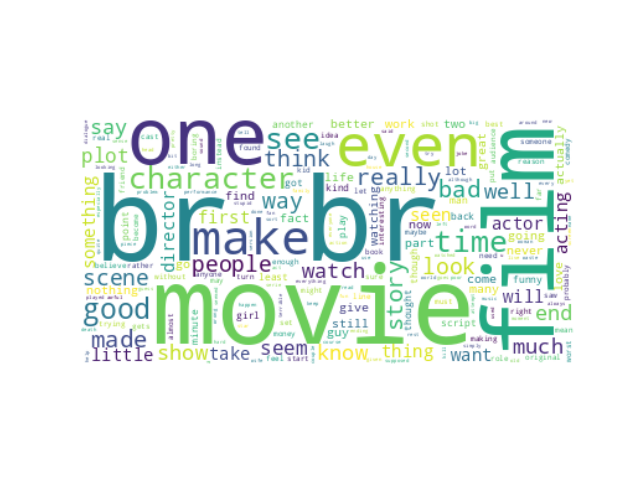
\includegraphics[width=\linewidth]{NegativeWordCloud.png}
  \caption{Negative Reviews Word Cloud}
  \label{fig1A}
\end{figure}
\\

\subsection{Random and Positive Guessing Models}

\subsubsection{Random Prediction Model}
The probability of predicting a new review to be positive or negative is $\frac{1}{2}$ as it equally probable to guess a particular review to be of correct type.  Here, in the given test samples we get the accuracy as $50.1933333333333\%$ which is quite close to $50\%$ implying both reviews are nearly equally likely in this data sample. 

\subsubsection{Positive Guessing Model}
Here, the probability depends on the test samples i.e. which are types of reviews are more likely and hence changing the probability. in the given test samples we get the accuracy as $66.66666666666666\%$ signifying that it is more likely to get a positive review compared to a negative review.

\subsubsection{Analysing Accuracy of different Models}
It is quite evident that both of the above model are very bad for predicting that a review is positive or negative. Our model gives the following improvement in accuracy over the above given models:
\begin{enumerate}
  \item Improvement in accuracy over the random prediction model: $82.91333333333333\%-50.1933333333333\%=32.720\%$.
  \item Improvement in accuracy over the random prediction model: $82.91333333333333\%-66.66666666666666\%=16.24666666666667\%$
\end{enumerate}

\subsubsection{Confusion Matrix}
\subsubsubsection{Confusion Matrix for different Models are as follows:}\\
The confusion matrix for our trained model is:
$$\begin{bmatrix}

11753 & 525 \\

747 & 11975 \
% [[11753   525]
%  [  747 11975]]
\end{bmatrix}$$
\\
The confusion matrix for random prediction model is:
$$\begin{bmatrix}

5023 & 2494 \\

4977 & 2506 \
% [[5023 2494]
%  [4977 2506]]
\end{bmatrix}$$
\\

The confusion matrix for Positive guessing model is:
$$\begin{bmatrix}

10000 & 5000 \\

0 & 0 \
% [[10000  5000]
%  [    0     0]]
\end{bmatrix}$$
\\

The confusion matrix given by our model as highest diagonal entry if we see per 100 examples (i.e percentage) and its denotes the accuracy of our model which is number of samples cases correctly guessed by our model is the accuracy for that model.
\\

We can observe that the True Positive value of all the matrices is the maximum among all the entries implying that all the models are majorly predicting the positive to be correct. Also in our model the false negative error is more than the false positive in the confusion matrix, thus the model is predicting more positive reviews to be negative than the negative reviews to be positive.
\\

In the positive guessing model, no positive review is wrong predicted because it is simply saying all reviews to be positive, therefore no negative, hence no positive being wrong predicted.

\subsection{Stemming and excluding Stopwords}
The results of stemming and excluding Stopwords the \texttt{test data} are:
\begin{enumerate}
  \item The training data accuracy is $95.56666666666666\%$
  \item The test data accuracy is $83.56666666666666\%$
\end{enumerate}
Here, we observe that both the training accuracy  and the testing accuracy increases because of removing usual words and adjusting similar words.

\begin{figure}[H]
  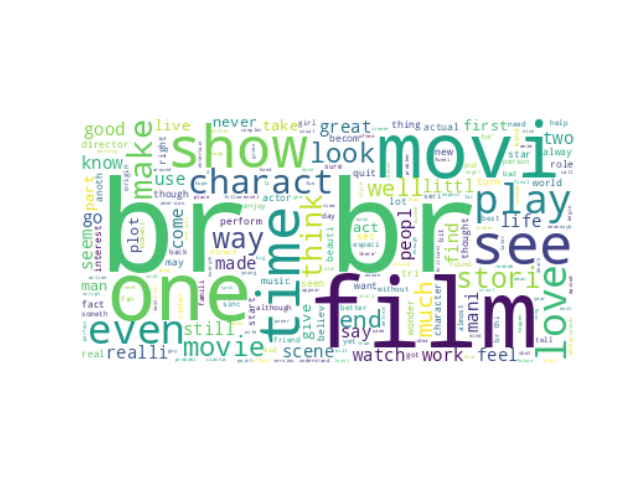
\includegraphics[width=\linewidth]{StemmedPositiveWordCloud.png}
  \caption{Positive Reviews Word Cloud with Stemming}
  \label{fig1A}
\end{figure}
\subsection{Random and Positive Guessing Models}
\\
\begin{figure}[H]
  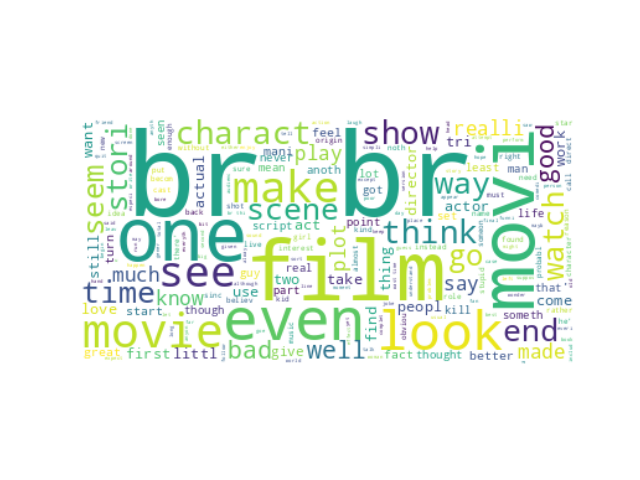
\includegraphics[width=\linewidth]{StemmedNegativeWordCloud.png}
  \caption{Negative Reviews Word Cloud with Stemming}
  \label{fig1B}
\end{figure}
\\

\subsection{Feature Engineering}

\subsubsection{Bigram over unigrams without stemming}
\begin{enumerate}
  \item The training data accuracy is $99.724\%$
  \item The test accuracy is $86.313\%$
\end{enumerate}
The training accuracy improves significantly because while using bigram over unigrams, we are basically over fitting the data. Contrary, there is a very slight increase in the accuracy of test data set as model learns quite low in general.

\subsubsection{Bigrams over unigrams + Stemming}
\begin{enumerate}
  \item The training data accuracy increases to $99.956\%$
  \item The test data accuracy is $85.713\%$
\end{enumerate}
With stemming the training data accuracy further increases possibly due the frequency of similar occurring words in training data but the test data accuracy decreases as it overfits to the data taking into account the very details in training data.
\subsubsection{TriGrams over Bigrams over unigrams + Stemming}
\begin{enumerate}
  \item The training data accuracy is $100\%$
  \item The test accuracy is $86.0\%$
\end{enumerate}
The training accuracy improves to 100 percent because we learning more and more on training data and trying to match the test data more and more with training data. Here, the test accuracy also increases with small amount as the test may be in resemblence with the training data. Further moving on to QuadGrams, it will lead to more and more overfitting leading to decrease in test accuracy and learning more and more on training data.
\subsubsection{Analysis of different features}
\begin{enumerate}
  \item The stemming increases the accuracy because the model is randomly distrubed by the different forms of different and hence was more dependent on the training and test data. After stemming our model becomes less sensitive to given data.  
  \item Performing bi-grams takes into the account the probability of occurring of a word after a particular word (conditional probability) which increases the accuracy on training data and here, in our case test accuracy also increases which implies that the words are dependent on the previous words and there is some probability related with words occurring in specific sequence.
  \item TriGrams further improves accuracy on training data set by overfitting on training data and taking into account conditional probabilities of three consecutive words. 
\end{enumerate}
\subsubsection{Comparison with models of previous parts}
\begin{enumerate}
  \item The initial model is working quite fine on the training and test data both.
  \item The stemming model increases the accuracy by 2 percent because stemming decreases the different forms of same word to a same word.
  \item BiGrams over stemming further improves the test accuracy to about 86 percent.
  \item BiGrams without stemming improves the test accuracies to shoot above 86 percent. It may be happening because of the occurrence of a specific form of a word after a particular word in a specific class (positive review or negative review class).
\end{enumerate}
\subsection{Precision, Recall and F1 Score}
\subsubsection{First Model without stemming}
The Precision, Recall and F1 Score for the first model is as follows:
\begin{enumerate}
  \item Precision is $0.9152428810720268\%$
  \item Recall is $0.8196\%$
  \item F1 Score is is $0.8647850171458717\%$
\end{enumerate}
\subsubsection{Model with stemming}
The Precision, Recall and F1 Score for the first model is as follows:
\begin{enumerate}
  \item Precision is $0.9196836359585607\%$
  \item Recall is $0.8256\%$
  \item F1 Score is is $0.8701059176898351\%$
\end{enumerate}
\subsubsection{Model with BiGrams + Stemming}
The Precision, Recall and F1 Score for the first model is as follows:
\begin{enumerate}
  \item Precision is $0.9334657398212513\%$
  \item Recall is $0.846\%$
  \item F1 Score is is $0.8875832765042228\%$
\end{enumerate}

% Summary field has been incorporated as weighted sum of the frequencies from \texttt{review text} and \texttt{summary} fields. Cleaning $+$ stemming was done before computation. The accuracy obtained is $65.93571428571429\%$ and the f1 score is $0.35236362262920623$. This model performs the best compared to all other models since the accuracy is also relatively higher and the f1 score is the highest of all models.
\subsubsection{Analysing the above metrics}
F1 Scores performs the best because it takes into account contribution from both precision and recall. Hence F1 score is more general and best among all the metrics.

\section{ Binary Image Classification}
\begin{itemize}
    \item \large Libraries Used
    \begin{itemize}
        \item[\ding{227}] os
        \item[\ding{227}] sys
        \item[\ding{227}] time
        \item[\ding{227}] numpy
        \item[\ding{227}] pickle
        \item[\ding{227}] sklearn.svm
        \item[\ding{227}] cvxopt
        \item[\ding{227}] cvxopt.solvers
    \end{itemize}
\end{itemize}
\subsection{Binary Classification}
Here in this problem, I'm using the RBG image of size $32 \times 32 \times 3$ to form a vector of length $3072$ and then classifying the images into two classes using SVMs. My entry number ends with $1$ and therefore the classes considered are $1$ and $2$ in the Support Vector Machine.

\subsubsection{Using Linear Kernel}
We are using the CVXOPT package, we need to first transform the dual problem into the CVXOPT API acceptable form
\begin{equation}
  \begin{split}
    &\alpha^T P \alpha + q^T \alpha + d\\
    &G \alpha \preceq H\\
    &A \alpha = b
  \end{split}
\end{equation}
The dual in summation format is given as:
\begin{equation}
  \frac{1}{2}\sum_{i=1}^m\sum_{j=1}^m \alpha_i \alpha_j y^i y^j (x^i)^T x^j - \sum_{i=1}^m \alpha_i
\end{equation}

It is easy to see that $P_{ij}$ is the coefficient of $\alpha_i \alpha_j$. Therefore, $P_{ij}$ is given as:
\begin{equation}
  \begin{split}
    &P_{ij} = y^i y^j (x^i)^T x^j\\
    \implies &P = X_y\times X_y^T\\
    \text{where }&X_y = \text{each row of }X\text{ multiplied by }Y
  \end{split}
\end{equation}
Also, $d$ is $0$ and $q$ is a vector with all $-1$:
\begin{equation}
  \begin{bmatrix}
    -1\\
    -1\\
    \vdots\\
    -1
  \end{bmatrix}
\end{equation}
The condition on $\alpha_i$ is $0 \leq \alpha_i \leq c$. Therefore $G$ and $H$ are given as:
\begin{equation}
  \begin{split}
    G &=
    \begin{bmatrix}
      -1 & 0 & \ldots & 0\\
      0 & -1 & \ldots & 0\\
      \vdots & \vdots & \ddots & \vdots\\
      0 & 0 & \ldots & -1\\
      1 & 0 & \ldots & 0\\
      0 & 1 & \ldots & 0\\
      \vdots & \vdots & \ddots & \vdots\\
      0 & 0 & \ldots & 1\\
    \end{bmatrix}\\
    H &=
    \begin{bmatrix}
      0\\
      0\\
      \vdots\\
      0\\
      c\\
      c\\
      \vdots\\
      c
    \end{bmatrix}
  \end{split}
\end{equation}
The equality condition is $\sum_{i=1}^m \alpha_i y^i = 0$. Therefore $A$ and $b$ are given as:
\begin{equation}
  \begin{split}
    A &=
    \begin{bmatrix}
      y_1 & y_2 & \ldots & y_m
    \end{bmatrix}\\
    b &= 0
  \end{split}
\end{equation}
% We now compute these values and pass them to the CVXOPT quadratic program solver. The results obtained are:
In this format, we pass them to the CVXOPT quadratic program solver and we got these results:
% \begin{equation}
%   \begin{split}
%     \text{training time }&= 26.060819149017334s\\
%     nSV &= 126\\
%     b &= 0.29323351252380514\\
%     \text{training accuracy }&= 100\%\\
%     \text{test accuracy }&=98.99446958270488\%
%   \end{split}
  
% \end{equation}
\begin{enumerate}
  \item Training Time:  $16.70463514328003$ seconds
  \item Number of support vectors in Class 1 are  826.0
  \item Number of support vectors in Class 1 are  826.0
  \item Number of support vectors in Class 2 are  721.0
  \item Total Number of support vectors in Class 2 are  1547.0
  \item Support Vector percentage in training examples is  38.675 $\%$
  \item w for linear kernel is:
  \begin{bmatrix}
      $-0.74565394$\\
      $0.03278262$\\
      $-0.48368186$\\
      \vdots\\
      $-0.09051983$\\
      $0.09775812$ \\
      $-1.04531297$
    \end{bmatrix}
  % \item No. of support vectors in Class 2 are  936.0
  \item b for linear kernel is : $-0.01833718$
  \item Testing Time over training data set:$  0.7171199321746826$ seconds
  \item Testing Time over testing data set:  $0.39896464347839355$ seconds
  \item The accuracy over training data is:  $94.875 \%$
  \item The accuracy over test data is:  $78.10000000000001 \%$
\end{enumerate}
The support vector images corresponding to the top-5 coefficients are as follows:
\begin{figure}[H]
\begin{center}
  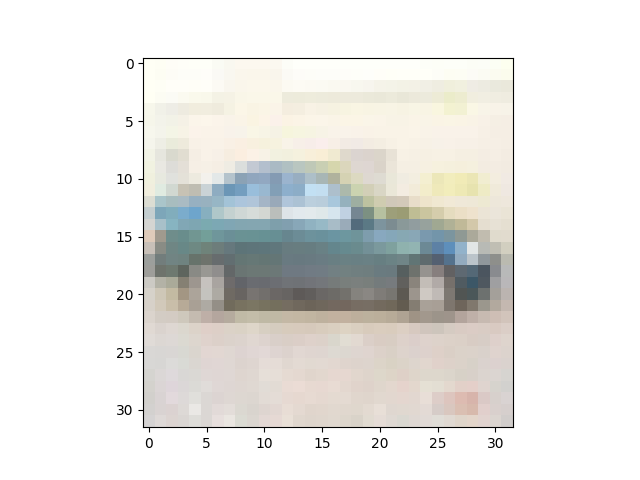
\includegraphics[scale=0.45]{a1.png}
  \caption{Support Vector A1}
  \label{fig2A}
\end{center}
\end{figure}
\begin{figure}[H]
\begin{center}
  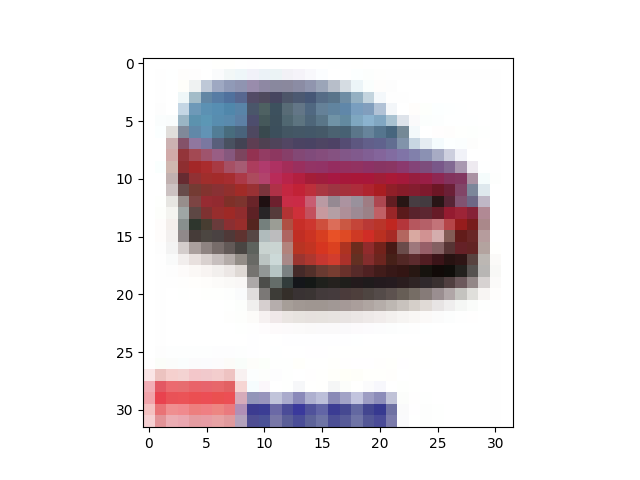
\includegraphics[scale=0.45]{a2.png}
  \caption{Support Vector A2}
  \label{fig2B}
\end{center}
\end{figure}
\begin{figure}[H]
\begin{center}
  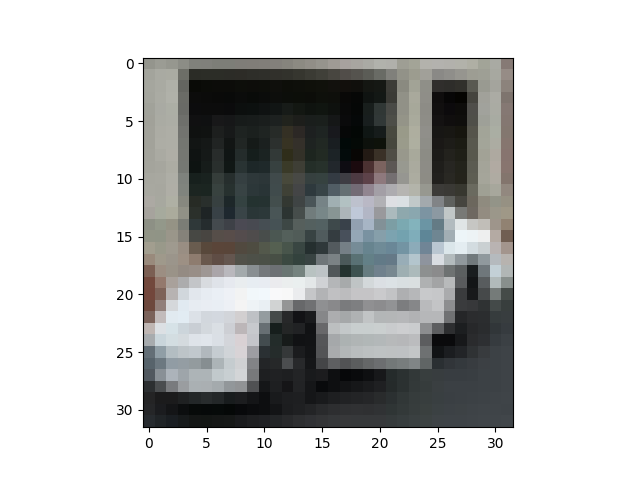
\includegraphics[scale=0.45]{a3.png}
  \caption{Support Vector A3}
  \label{fig2C}
\end{center}
\end{figure}
\begin{figure}[H]
\begin{center}
  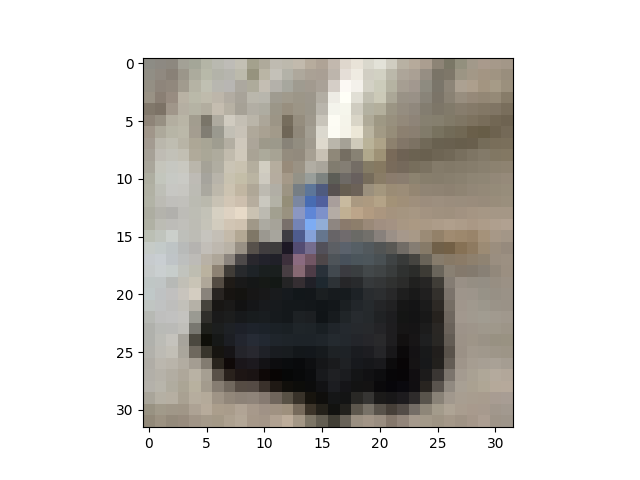
\includegraphics[scale=0.45]{a4.png}
  \caption{Support Vector A4}
  \label{fig2D}
\end{center}
\end{figure}
\begin{figure}[H]
\begin{center}
  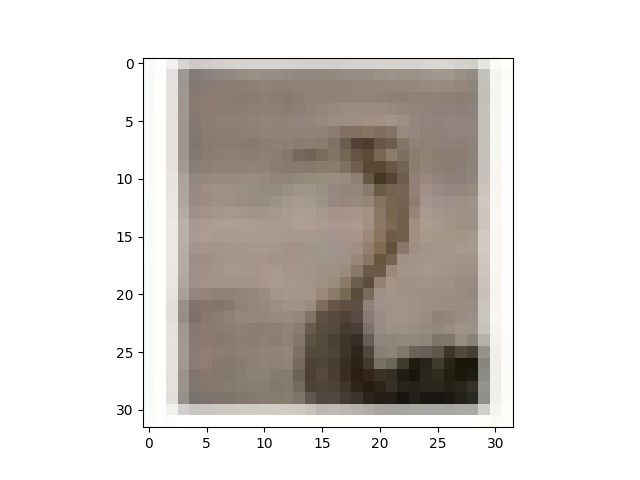
\includegraphics[scale=0.45]{a5.png}
  \caption{Support Vector A5}
  \label{fig2E}
\end{center}
\end{figure}
\\
The Plot w (weight) vector is as follows:
\begin{figure}[H]
\begin{center}
  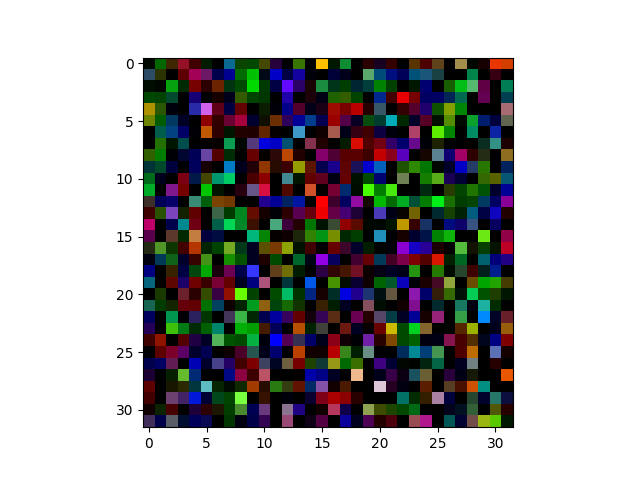
\includegraphics[scale=0.45]{w.png}
  \caption{w (weight) Vector}
  \label{fig2F}
\end{center}
\end{figure}

\subsection{Using Gaussian Kernel}
The dual SVM problem transforms as following if use the guassian kernel:
\begin{equation}
  \text{min}(- \sum_{i=1}^m \alpha_i + \frac{1}{2}\sum_{i=1}^m\sum_{j=1}^m \alpha_i \alpha_j y^i y^j \phi(x^i)^T \phi(x^j))
\end{equation}
The only difference will be in the value of $P$, and $P$ is given as:
\begin{equation}
  \begin{split}
    &P_{ij} = y^i y^j \phi(x^i)^T \phi(x)^j\\
    \implies &P_{ij} = y^i y^j \exp(-\gamma ||x^i - x^j||^2)\\
    \implies &P_{ij} = y^i y^j \exp(-\gamma (||x^i||^2 + ||x^j||^2 - 2 x^i x^j))
  \end{split}
\end{equation}
We generalise this equation for computing the \textit{product} of any two vectors $X, Z$ of sizes $n,m$ respectively as:
\begin{equation}
  \mathcal{P}(X, Z) =
  \begin{bmatrix}
    ||X_1||^2 & ||X_1||^2 & (m \text{ times})\ldots & ||X_1||^2\\
    ||X_2||^2 & ||X_2||^2 & (m \text{ times})\ldots & ||X_2||^2\\
    \vdots & \vdots & \ddots & \vdots\\
    ||X_n||^2 & ||X_n||^2 & (m \text{ times})\ldots & ||X_n||^2
  \end{bmatrix} +
  \begin{bmatrix}
    ||Z_1||^2 & ||Z_2||^2 & \ldots & ||Z_m||^2\\
    ||Z_1||^2 & ||Z_2||^2 & \ldots & ||Z_m||^2\\
    \vdots & \vdots & & \vdots\\
    n\text{ times} & n\text{ times} & \ddots & n\text{ times}\\
    \vdots & \vdots & & \vdots\\
    ||Z_1||^2 & ||Z_2||^2 & \ldots & ||Z_m||^2
  \end{bmatrix} -
  2 (X \otimes Z)
\end{equation}
This type of formulation is made to solve the Gaussian kernel using the numpy methods. The values are then again passed to the CVXOPT quadratic problem solver. We make predictions as:
\begin{equation}
  (\alpha \times Y) \times \exp(-\gamma \mathcal{P}(X_{SV}, X_{data})) + b
\end{equation}
The following are the results obtained:
\begin{enumerate}
  \item Training Time:  $15.430006265640259$ seconds
  \item Number of support vectors in Class 1 are  945.0
  \item Number of support vectors in Class 2 are  936.0
  \item Total Number of support vectors in Class 2 are  1881.0
  \item Support Vector percentage in training examples is  47.025 $\%$
  % \item No. of support vectors in Class 2 are  936.0
  \item The accuracy over test data is:  $82.1 \%$
\end{enumerate}

The accuracy obtained here is approximately 4 percent more than the model trained using cvxopt package implying scikit trains better than cvxopt package.
\\
\\

The support vector images corresponding to the top-5 coefficients are as follows:
\begin{figure}[H]
\begin{center}
  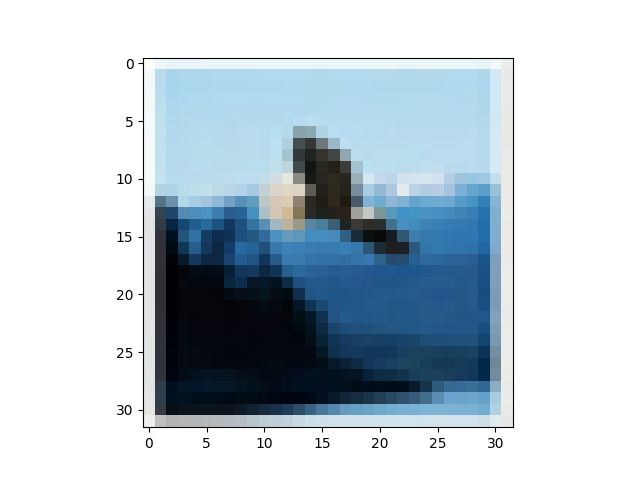
\includegraphics[scale=0.45]{b1.png}
  \caption{Support Vector B1}
  \label{fig3A}
\end{center}
\end{figure}
\begin{figure}[H]
\begin{center}
  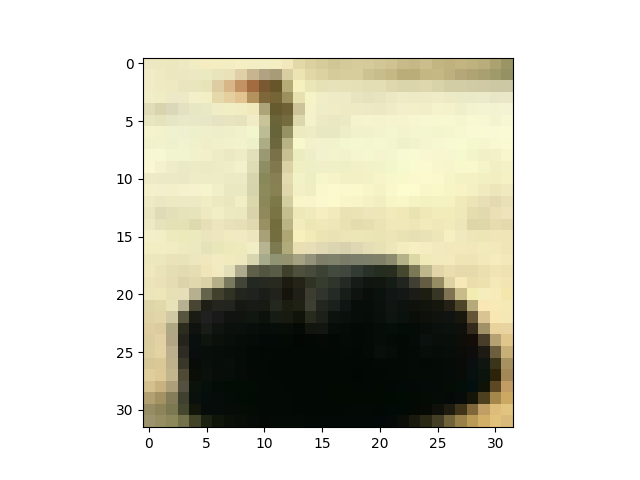
\includegraphics[scale=0.45]{b2.png}
  \caption{Support Vector B2}
  \label{fig3B}
\end{center}
\end{figure}
\begin{figure}[H]
\begin{center}
  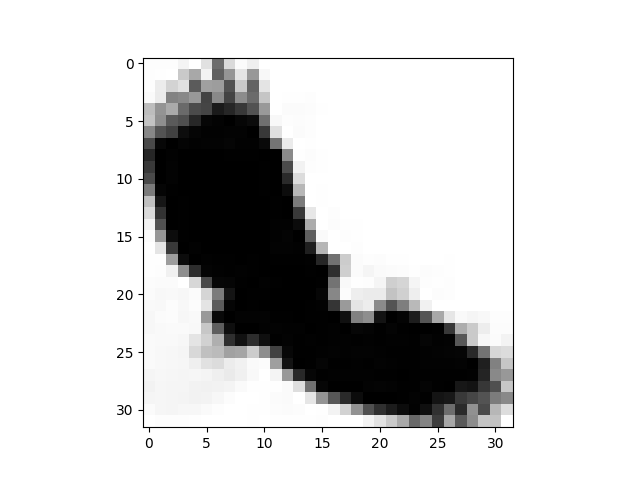
\includegraphics[scale=0.45]{b3.png}
  \caption{Support Vector B3}
  \label{fig3C}
\end{center}
\end{figure}
\begin{figure}[H]
\begin{center}
  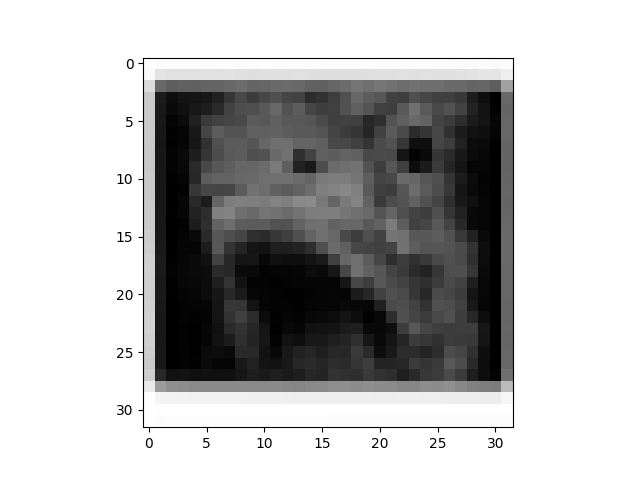
\includegraphics[scale=0.45]{b4.png}
  \caption{Support Vector B4}
  \label{fig3D}
\end{center}
\end{figure}
\begin{figure}[H]
\begin{center}
  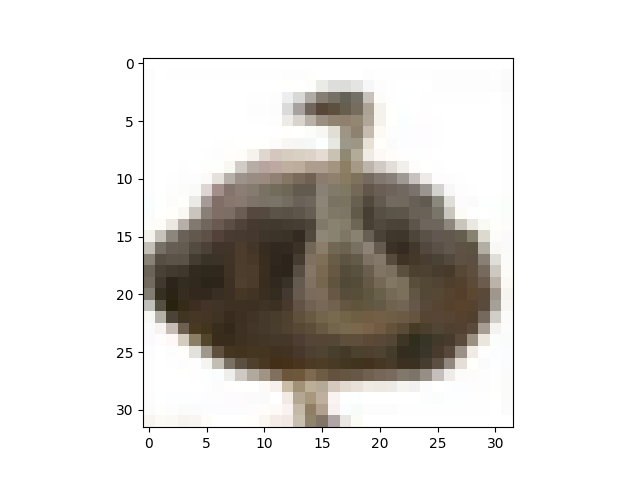
\includegraphics[scale=0.45]{b5.png}
  \caption{Support Vector B5}
  \label{fig3E}
\end{center}
\end{figure}
\\

\subsection{Using scikit learn SVM function, based on LIBSVM package}

\paragraph{Linear Kernel}
The results are as follows:
\begin{enumerate}
  \item Time taken to train with Linear kernel by scikit:  $17.533120155334473$ seconds
  \item No. of Support Vectors in Class 1 are 822
  \item No. of Support Vectors in Class 2 are 719
  \item Total Number of support vectors in Class 2 are  1541
  \item Support Vector percentage in training examples is  38.525 $\%$
  \item w for linear kernel is:
  \begin{bmatrix}
      $-0.74586634$\\
      $0.03277407$\\
      $-0.48379131$\\
      \vdots\\
      $-0.09057429$\\
      $0.09792686$ \\
      $-1.04533378$
    \end{bmatrix}
    \item b for linear kernel is : $0.01147231  $
  % \item No. of support vectors in Class 2 are  936.0
  \item The accuracy over test data is:  $78.05 \%$
\end{enumerate}

\paragraph{Gaussian Kernel}
The results are as follows:
\begin{enumerate}
  \item Time taken to train with Gaussian kernel by scikit:  $11.59799337387085$seconds
  \item Number of support vectors in Class 1 are 939
  \item Number of support vectors in Class 2 are 926
  \item Total Number of support vectors (nSV) are  1865
  \item Support Vector percentage in training examples is  46.625 $\%$
  \item The accuracy over test data is:  $87.4 \%$
\end{enumerate}

\paragraph{Training Time Comparison}
    \begin{itemize}
        \item The scikit uses approximately 1 second more than cvxopt to train the model with linear kernel, scikit takes slightly more and trains upto less error.
        \item The scikit uses approximately 4 second more than cvxopt to train the model with gaussian kernel, scikit is relatively slow than cvxopt and requires more time when more computation is there.
    \end{itemize}
\section{Multi-Class Image Classification}
\begin{itemize}
    \item \large Libraries Used
    \begin{itemize}
        \item[\ding{227}] os
        \item[\ding{227}] sys
        \item[\ding{227}] time
        \item[\ding{227}] numpy
        \item[\ding{227}] pickle
        \item[\ding{227}] cvxopt
        \item[\ding{227}] cvxopt.solvers
        \item[\ding{227}] sklearn.svm
        \item[\ding{227}] random
    \end{itemize}
\end{itemize}
\subsection{One vs One Classifier using CVXOPT package (Gaussian kernel is Used)}
The Class with maximum number of votes is considered as predicted class. In case of ties, the label with highest score is chosen.\\
The results are as follows:
\begin{enumerate}
  \item Training Time over all classes by  cvxopt:  $168.1200668811798$ sec
  \item The accuracy over test data is:  $57.02 \%$
\end{enumerate}

\subsection{One vs One Classifier using Scikit Learn SVM LIBSVM package (Gaussian kernel is Used)}
The results are as follows:
\begin{enumerate}
  \item Training Time over classes by scikit:  $130.7175416946411$ sec
  \item The accuracy over test data is:  $59.3 \%$
\end{enumerate}
% The training time is much lesser than using CVXOPT (takes $\frac{1}{5}$ the time), however the prediction time is larger with the model that is trained by LIBSVM (takes $6 \times$ time).
The training time is quite less while scikit which trains in approximately 38 seconds before the cvxopt. Here, it is quite clear that scikit faster than cvxopt in multi class classification.
\subsection{Confusion Matrix}
The confusion matrix using CVXOPT is:
\begin{equation}
  \begin{bmatrix}
    724 & 121 & 135 & 79 & 75\\
    46 & 562 & 23 & 32 & 18\\
    101 & 87 & 457 & 128 & 283\\
    75 & 193 & 214 & 684 & 200\\
    54 & 37 & 171 & 77 & 424
  \end{bmatrix}
\end{equation}
\\
\paragraph{Observation}
\begin{itemize}
    \item The trace of the confusion matrix corresponds to correct prediction and rest all are the wrong predictions.
    \item Many Birds are wrongly classified as Cat or Deer. Also more of deer are wrongly classified as cat or bird.
\end{itemize}
\\
The confusion matrix using LIBSVM is:
\begin{equation}
  \begin{bmatrix}
    729 & 100 & 145 & 82 & 98\\
    83 & 731 & 61 & 97 & 48\\
    78 & 42 & 409 & 123 & 212\\
    61 & 92 & 133 & 572 & 118\\
    49 & 35 & 252 & 126 & 524
  \end{bmatrix}
\end{equation}
\\
\begin{itemize}
    \item Scikit also gives quite similar results. More of Birds are classified as deer in the case of scikit model.
    \item Scikit trained model also gives more accuracy over the test data.
\end{itemize}
\\
\newpage
The 10 misclassified examples by cvxopt package are as follows:
\begin{figure}[H]
    \begin{subfigure}[b]{0.3\textwidth}
        \centering
        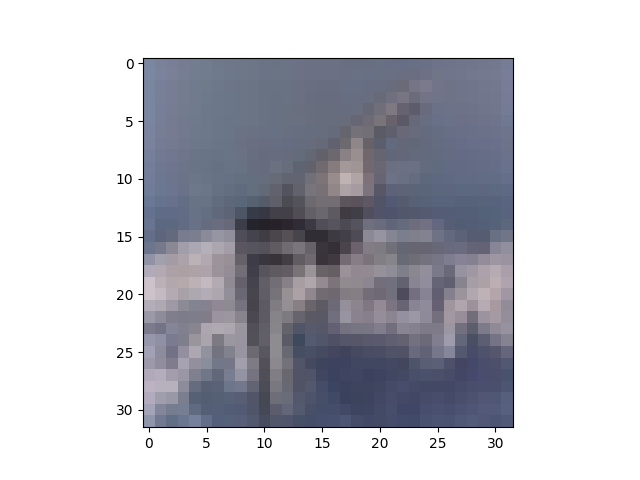
\includegraphics[width=\linewidth]{misA1.png}
        \caption{Example 1: Predicted Aeroplane(Bird)}
    \end{subfigure} 
    % \hfill
    \begin{subfigure}[b]{0.3\textwidth}
        \centering
        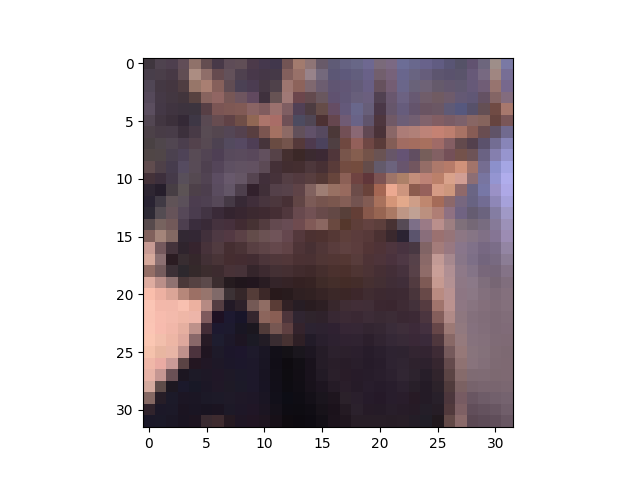
\includegraphics[width=\linewidth]{misA2.png}
        \caption{Example 2: Predicted Bird(Deer)}
    \end{subfigure} 
    % \hfill
    \begin{subfigure}[b]{0.3\textwidth}
        \centering
        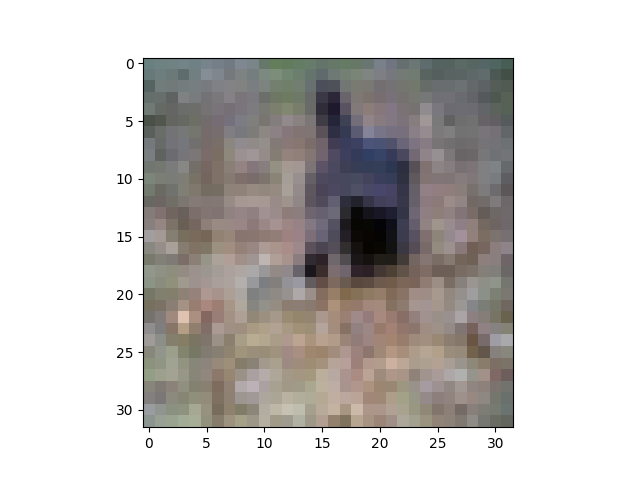
\includegraphics[width=\linewidth]{misA3.png}
        \caption{Example 3: Cat(Bird)}
    \end{subfigure} 
    \medskip
    \begin{subfigure}[b]{0.3\textwidth}
        \centering
        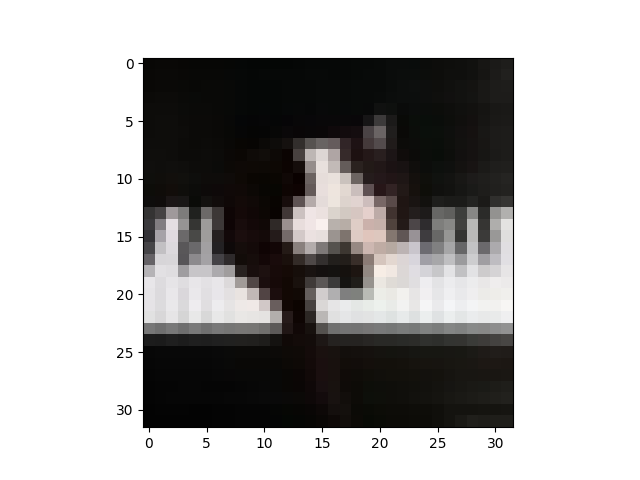
\includegraphics[width=\linewidth]{misA4.png}
        \caption{Example 4: Predicted Aeroplane(Bird)}
    \end{subfigure}
    % \hfill
    \begin{subfigure}[b]{0.3\textwidth}
        \centering
        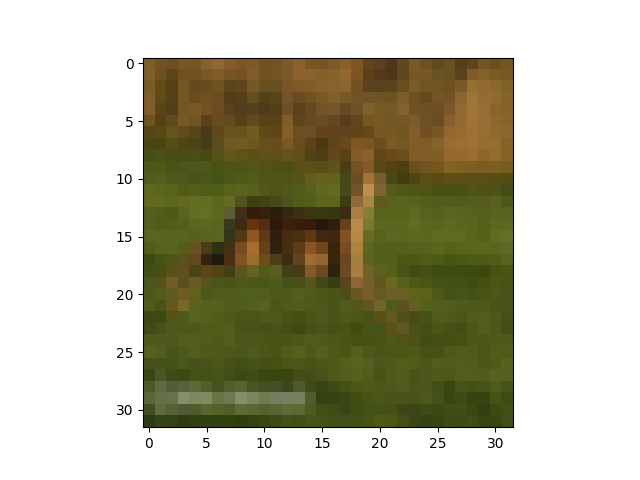
\includegraphics[width=\linewidth]{misA5.png}
        \caption{Example 5: Predicted Bird(Deer)}
    \end{subfigure}
    % \hfill
    \begin{subfigure}[b]{0.3\textwidth}
        \centering
        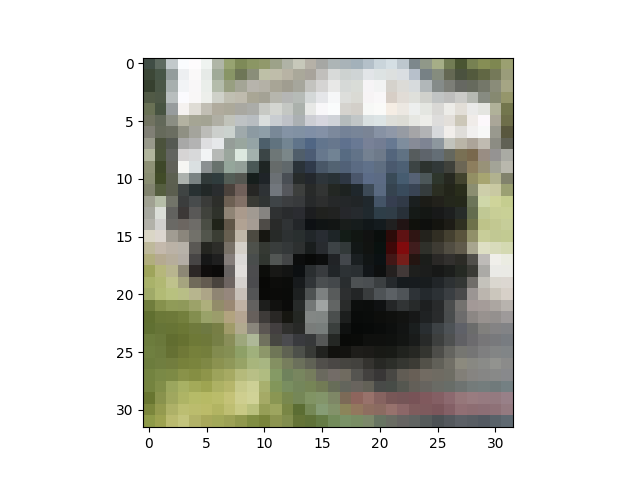
\includegraphics[width=\linewidth]{misA6.png}
        \caption{Example 6: Predicted Deer(Car)}
    \end{subfigure} 
    \medskip
    \begin{subfigure}[b]{0.3\textwidth}
        \centering
        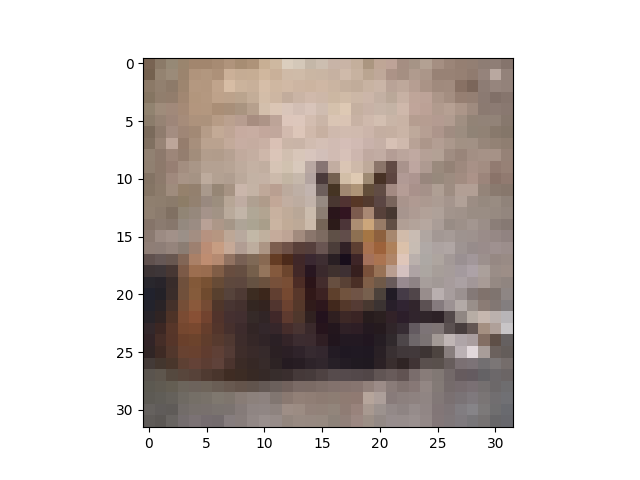
\includegraphics[width=\linewidth]{misA7.png}
        \caption{Example 7: Predicted Deer(Cat)}
    \end{subfigure}
    \hfill
    \begin{subfigure}[b]{0.3\textwidth}
        \centering
        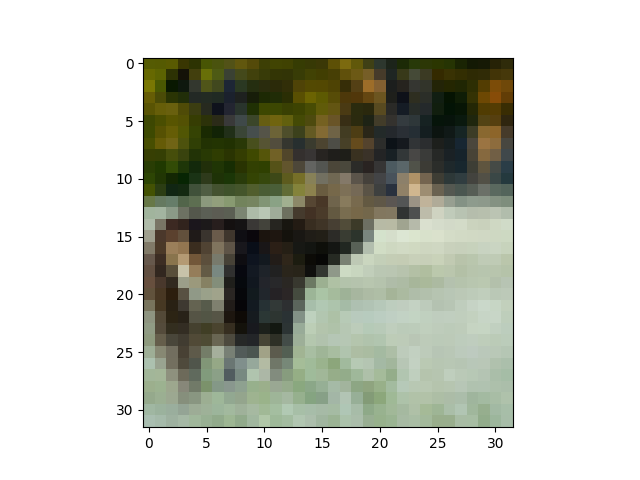
\includegraphics[width=\linewidth]{misA8.png}
        \caption{Example 8: Predicted Bird(Deer)}
    \end{subfigure} 
    \hfill
    \begin{subfigure}[b]{0.3\textwidth}
        \centering
        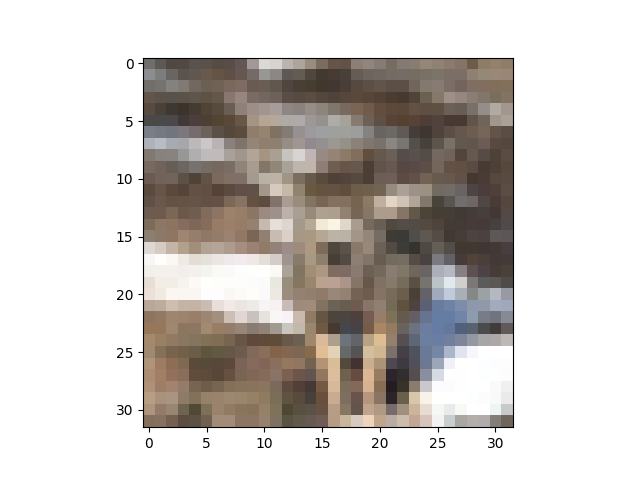
\includegraphics[width=\linewidth]{misA9.png}
        \caption{Example 9: Predicted Bird(Deer)}
    \end{subfigure}
    \hfill
    \begin{subfigure}[b]{0.3\textwidth}
        \centering
        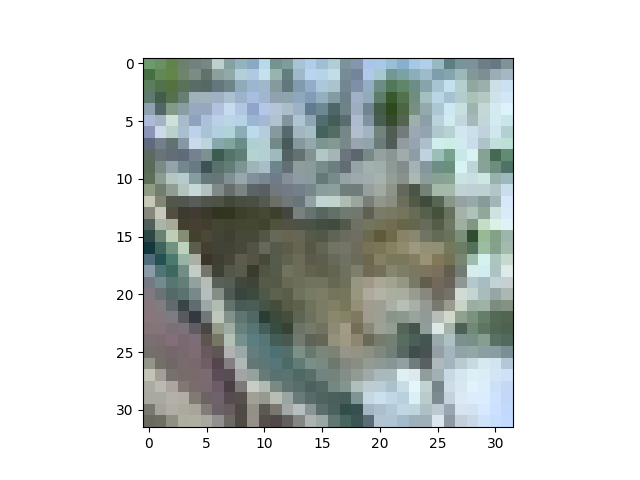
\includegraphics[width=\linewidth]{misA10.png}
        \caption{Example 10: Predicted Cat(Deer)}
    \end{subfigure} 
    % \caption{Misclassifications by the model}
\end{figure}
\newpage
The 10 misclassified examples by scikit package are as follows:
\begin{figure}[H]
    \begin{subfigure}[b]{0.3\textwidth}
        \centering
        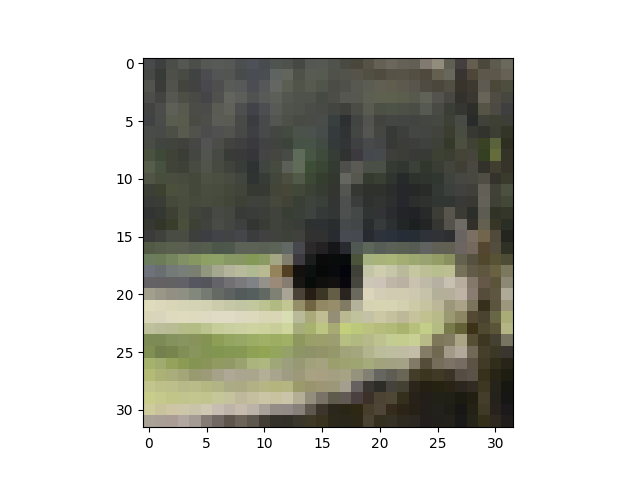
\includegraphics[width=\linewidth]{misB1.png}
        \caption{Example 1: Predicted Cat(Bird)}
    \end{subfigure} 
    % \hfill
    \begin{subfigure}[b]{0.3\textwidth}
        \centering
        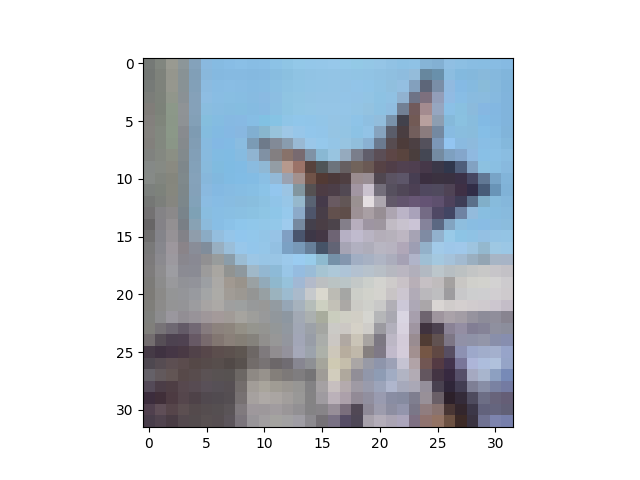
\includegraphics[width=\linewidth]{misB2.png}
        \caption{Example 2: Predicted Aeroplane(Cat)}
    \end{subfigure} 
    % \hfill
    \begin{subfigure}[b]{0.3\textwidth}
        \centering
        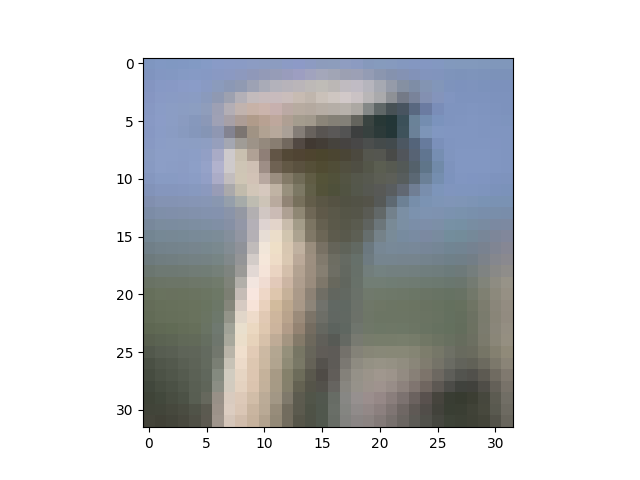
\includegraphics[width=\linewidth]{misB3.png}
        \caption{Example 3: Predicted Cat(Bird)}
    \end{subfigure} 
    \medskip
    \begin{subfigure}[b]{0.3\textwidth}
        \centering
        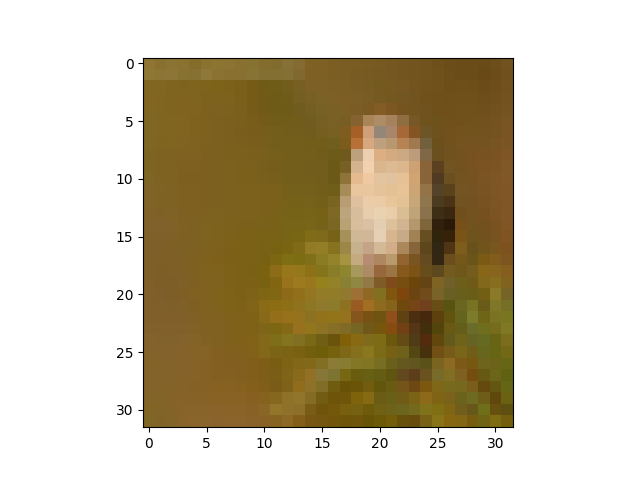
\includegraphics[width=\linewidth]{misB4.png}
        \caption{Example 4: Predicted Cat(Bird)}
    \end{subfigure}
    % \hfill
    \begin{subfigure}[b]{0.3\textwidth}
        \centering
        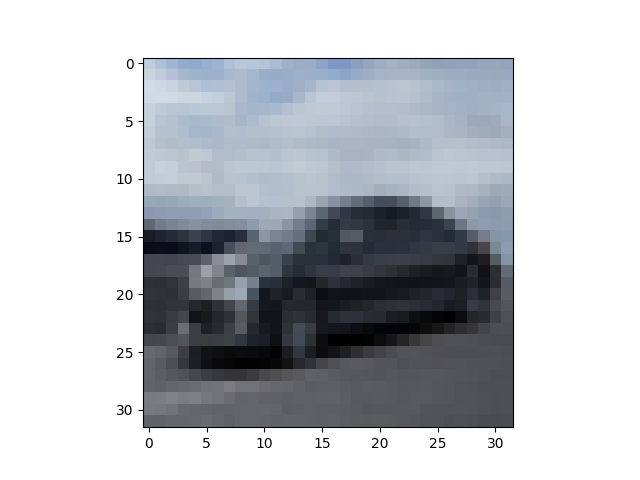
\includegraphics[width=\linewidth]{misB5.png}
        \caption{Example 5: Predicted Car(Cat)}
    \end{subfigure}
    % \hfill
    \begin{subfigure}[b]{0.3\textwidth}
        \centering
        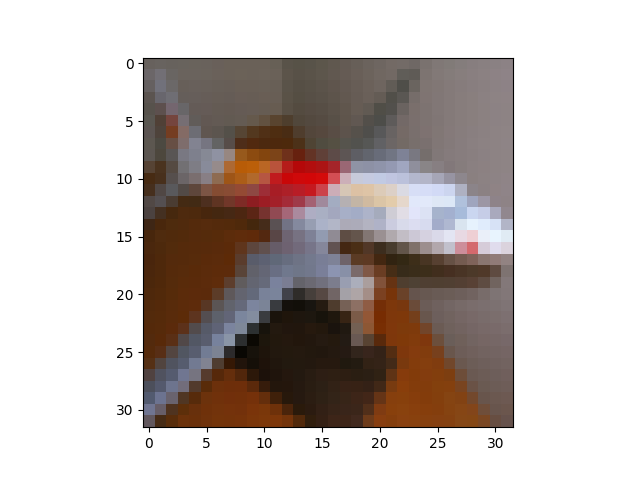
\includegraphics[width=\linewidth]{misB6.png}
        \caption{Example 6: Predicted Bird(Aeroplane)}
    \end{subfigure} 
    \medskip
    \begin{subfigure}[b]{0.3\textwidth}
        \centering
        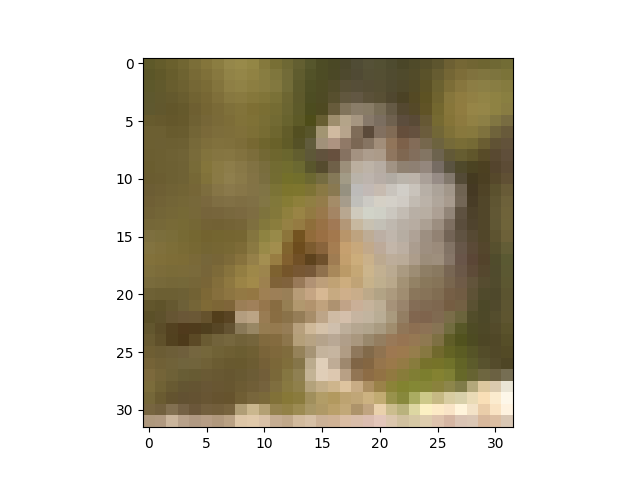
\includegraphics[width=\linewidth]{misB7.png}
        \caption{Example 7 :Predicted Bird(Cat)}
    \end{subfigure}
    \hfill
    \begin{subfigure}[b]{0.3\textwidth}
        \centering
        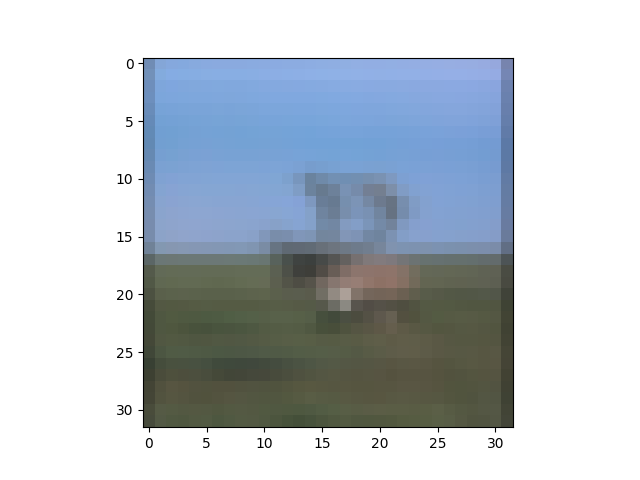
\includegraphics[width=\linewidth]{misB8.png}
        \caption{Example 8: Aeroplane(Deer)}
    \end{subfigure} 
    \hfill
    \begin{subfigure}[b]{0.3\textwidth}
        \centering
        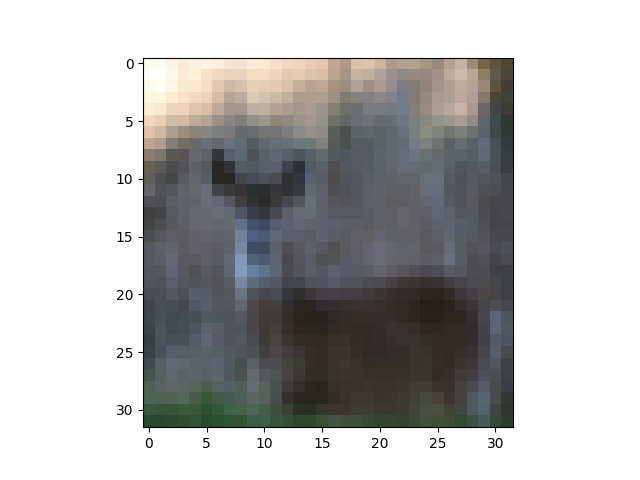
\includegraphics[width=\linewidth]{misB9.png}
        \caption{Example 9: Predicted Deer(Cat)}
    \end{subfigure}
    \hfill
    \begin{subfigure}[b]{0.3\textwidth}
        \centering
        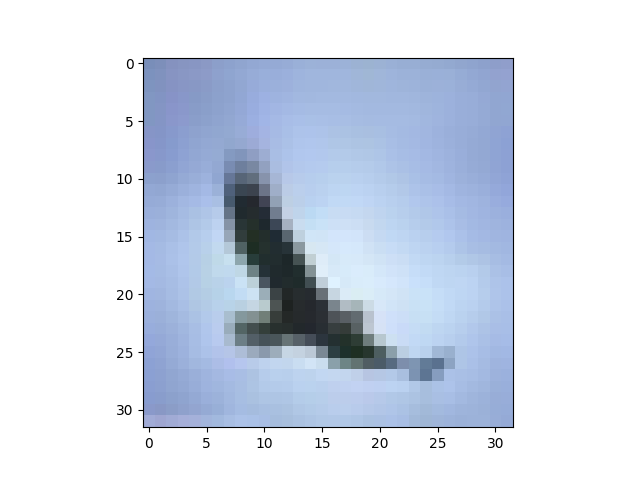
\includegraphics[width=\linewidth]{misB10.png}
        \caption{Example 10: Predicted Plane(Bird)}
    \end{subfigure} 
    % \caption{Misclassifications by the model}
\end{figure}
\newpage
% The misclassified data is submitted in the output directory of Q2. The reason for misclassification is because of the different styles of writing the number which leads to \textit{confusion} in identifying which digit the image represents.

\subsection{Cross-Validation and Regularization}
The 5-Fold Cross Validation was implemented with Sckit-learn's SVM model and one out of 5 division of training data is taken as Validation set. The Average of Validation set accuracies and test set accuracies are as follows:
\begin{center}
\begin{tabular}{c|c|c}
    
    % \hline
    
     C & Validation Accuracy & Test Accuracy  \\
    \hline
    $10^{-5}$ &  19.86\% & 20 \\
    $10^{-3}$ & 21.1\% & 27.36\%\\
    $1$ & 59.74\%& 60.54\% \\
    $5$ & 60.39\%& 61.44\\% \\
    $10$ & 61.57\% & 63.05\% \\
    
    
\end{tabular}
    
\end{center}
\begin{figure}[H]
    \centering
    \includegraphics[scale=1]{Accplot.png}
    \caption{Validation and Test Accuracy Graph}
\end{figure}
\begin{itemize}
    \item As seen in the graph, the validation accuracy peaks at $C = 10$, which also gives the highest accuracy in the test data. As a result, we can infer that the cross-validation approach is a reliable estimate for identifying the model's hyperparameters, which may help it perform at its peak during testing.
    \item With the lower values of $C$, there is huge relaxation on $\xi_i$, hence our model underfits on the training data set giving very less accuracy. With the increase in the value of $C$, there gets tighter on $\xi_i$ learning well on the training data and hence increasing accuarcy. Although, too high value of parameter $C$ leads to overfitting of the model on the training data and hence decreasing the test set accuracy.
    % \item From the primal problem of the SVM, we can deduce the for lower values of $C$, the model tends to have a high relaxation on $\xi_i$ and hence under-fits on the training data, resulting in low validation and test accuracies. On the other side, for high values of $C$, the model has a high penalty on the values of $\xi_i$ and results in a model that over-fits on the training data, and again dropping in accuracy. The model peaks in performance between under-fitting and over-fitting regions. This is all in compliance with the above experimental observations.

\end{itemize}

\end{document}